\section{Shared memory}
\label{sharedMemory}
The previous chapters introduced the means to enable parallel execution of code in terms of tasks and futures. Still missing is the communication between tasks. The communication model of choice for ParallelMbeddr is shared memory. The reason for this choice follows from the objectives for a communication model: it should offer a reasonable performance, considering that it is supposed to be used in embedded systems; it should be reasonably safe by design in order to avoid the trip hazards that are involved with low-level synchronization approaches like mutexes. Transactional memory seems to be not ready for the embedded domain for performance reasons. By following argumentation message passing does not offer profound advantages in comparison to shared memory if the access to the shared memory is controlled in a sane way. Usually message passing forbids shared memory between two parallel units of execution. Instead communication is realized via messages sends. A strict seperation of memory does not fit the usual C workflow concerning pointer arithmetic. Therefore some form of memory sharing would have to be introduced into a message passing model in order to reduce performance loss. As this would lead to the same problems that the general shared memory model already suffers from the opposite way is chosen: Instead of introducing shared memory in a message passing model a shared memory model is designed on top of which message passing can ever be attached in order to simplify the communication between tasks\footnote{Such an extension would be future concern and is not implemented in this work.}.

Memory that is to be shared between two tasks must be explicitly declared by an according type. A variable of this type denotes a \textit{shared ressource}. Thus, a shared ressource can be regarded as a wrapper of data that is to be shared. In order to make use of a shared ressource it has to be synchronized first. Specific language elements are used to access and change the value of a shared ressource. The chosen approach enables the programmer to use shared data both globally and locally and like any other data nest it inside structs and arrays. Additionally the new data type enables the IDE to ensure despite the arbitrary structuring of shared ressources that data is shared in a sane way.

\subsection{Design}
The ressources to be shared are typed with the shared ressource type:

$ t ::= ...|\;\mathit{shared{<}u{>}}\;|\;\mathit{shared{<}shared{<}u{>}{*}{>}}\;$

$ u ::= t \qquad u \neq t*$

The type parameterization denotes the base type of a shared type, i.e. the type of the data that is wrapped by a shared ressource. Due to reasons that will be explained in the SAFETY CHAPTER a shared ressource may have an arbitrary base type that does not denote a pointer to a value that is not shared\footnote{Differently said: A pointer wrapped in a shared ressource must point to a shared ressource itself. Due to the comprehensive type system that mbeddr is equipped with and that is only partially existant in C99 the compatibility of base types of shared types was mainly tested with the primitive types of C99 as well as pointer types, array types, struct types and type definitions (typedefs). Future work will have to be done to demonstrate and establish full compatibility with the rest of mbeddr's types.}. Further restrictions apply to shared types which are also investigated in the aforementioned section. The same applies to the \CODE{.set} expression by which the value of a shared ressource can be modified; the value can be retrieved via \CODE{.get}:

$ e ::= e.\mathit{get}\;|\;e.\mathit{set(e)} $
\begin{align*}
\inference*[SharedGet]{e |- \mathit{shared{<}t{>}}} {\quad e.\mathit{get} |- t \quad}
\qquad
\inference*[SharedSet]{e |- \mathit{shared{<}t{>}} \quad e' |- t' \quad t' <: t} {\qquad\quad e.\mathit{set}(e') |- \mathit{void} \quad\qquad} 
\end{align*}

The syntax \texttt{stmts} of statements in mbeddr is extended by the synchronization statement \CODE{sync} that contains a \textit{synchronization list} of shared ressources to synchronize over and a block of statements whose referenced shared ressources may be synchronized by a surrounding synchronization statement:

$ \mathit{stmt} ::= ...
        |\;\mathit{sync}(res, ..., res) \{\;\mathit{stmt} ... \mathit{stmt}\;\}$
        
\texttt{res} denotes the syntax of possible \textit{synchronization references}. Each synchronization reference \CODE{res} wraps a reference \CODE{e} to a shared ressource. \CODE{e} can either be of type \CODE{shared<t>} or of type \CODE{shared<t>*}. A shared ressource can be synchronized as is or be named by a synchronization reference:

$ res ::= e\;|\;e\;\mathit{as}\;[\mathit{resName}] $

The latter allows the programmer to refer to the result of an arbitrary complex expression which evaluates to a shared ressource inside the \CODE{sync} statement. Hence, a named ressource (i.e. a synchronization reference with a name for its referenced shared ressource) can be seen as syntactic sugar for a local variable declaration that binds a shared ressource to which a shared ressource reference evaluates. Due to the copy semantics of C the type of a named ressource \CODE{e} is restricted to \CODE{shared<t*>}. This enforcement ensures that the synchronized ressource is actually the original shared ressource and not a copy thereof over which a synchronization would be useless. The scope of a named ressource is restricted to the according synchronization statement. More precisely, a named ressource \textit{n} of a synchronization statement \textit{s} can be referenced from anywhere inside the abstract syntax tree (AST) of the statement list of \textit{s}. Furthermore it can be referenced from within the expression of any synchronization reference that follows \textit{n} in the synchronization list of \textit{s}, e.g.:
\begin{ccode}
shared<shared<int32>> v;
// vContent is declared before it is used in the list => valid
sync(v, &(v.get) as vContent, vContent->get as vContentContent) {
  vContentContent.set(0);
}
// vContentContent is not in scope, here => invalid
vContentContent.set(1);
\end{ccode}

The type of a reference to a named ressource is given by the corresponding shared ressource that is bound by the  synchronization reference.

In contrast to Java's synchronization blocks and methods\cite[p.~279]{JavaPerformanceTuning} the synchronization of tasks is not computation oriented but data oriented. The crucial difference is that a synchronized block \CODE{A} in Java is only protected against simultaneous executions by multiple threads. Thus, it is valid to access the data that is involved in \CODE{A} by some other computation whose protecting block (if any) is completely unrelated to \CODE{A}. Since low-level data races can obviously not be safely excluded with this scheme ParallelMbeddr ties the protection to the data that shall be shared. Every shared ressource is therefore protected seperately and application-wide. Concluding, consider two synchronization blocks which are about to be executed in parallel. If they contain synchronization references which overlap in terms of their referenced shared ressources their executions will be serialized. For instance take two tasks \textit{t1} and \textit{t2} that have access to the same shared ressource which is referenced by a global variable \CODE{value}. \textit{t1} wants to synchronize \CODE{value}, simultaneously \textit{t2} wants to synchronize \CODE{valuePointer} which points to \CODE{value}'s shared ressource and some other shared ressource that is available via the variable \CODE{other}:

\begin{ccode}
shared<int32> value;
shared<int32>* valuePointer = &value;
shared<double> other;
\end{ccode}
The synchronization semantics will then cause one thread to wait for the other to finish the execution of the blocking synchronization statement before it starts the execution of its own synchronization statement. The execution order might therefore be changed in the following manner:

\adjustbox{valign=t}{
\begin{minipage}{0.35\textwidth}
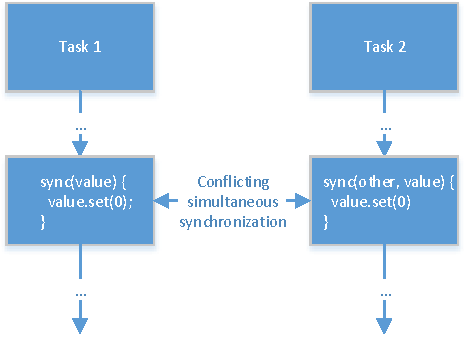
\includegraphics[scale=.9]{pics/ParallelExecutionAttempt}
\end{minipage}
}
\begin{minipage}{0.2\textwidth}
\begin{center}
\vspace{3.5cm}
\qquad\quad$\Longrightarrow$
\end{center}
\end{minipage}
\adjustbox{valign=t}{
\begin{minipage}{0.35\textwidth}
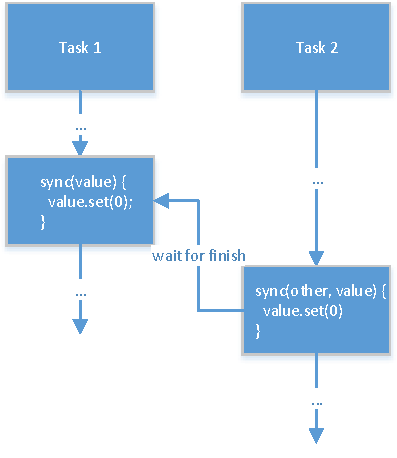
\includegraphics[scale=.9]{pics/SerialExecution}
\end{minipage}}

The possibility to refer to multiple shared ressources in the synchronization list of a synchronization statement is not mere syntactic sugar for nested synchronization statements. Instead the semantics of a synchronization list is that all referenced shared ressources are synchronized over at once, but with a possible time delay. By the design of the underlying implementation deadlocks by competing synchronization statements are thus avoided\footnote{Nevertheless deadlocks can obviously still occur if nested synchronization statements compete for the same ressources in an unsorted order.}.

As a result of the fact that generally the access to shared ressources is ressource-centric, a value wrapped in a shared ressource which in turn contains nested shared ressources is indepedently protected from the latter. Therefore a shared ressource of a struct with a shared member \CODE{b} is indepedently synchronized from \CODE{b}:

\vspace{0.5cm}
\begin{minipage}{0.35\textwidth}
\begin{ccode}
struct A {
  int32 a;
  shared<int32> b; 
}
shared<A> sharedA;
shared<int32>* sharedB;
sync(sharedA) { sharedB = &(sharedA.get.b); }
\end{ccode}
\end{minipage}
\begin{minipage}{0.2\textwidth}
\begin{center}
\qquad\quad$\Longrightarrow$
\end{center}
\end{minipage}
\begin{minipage}{0.35\textwidth}
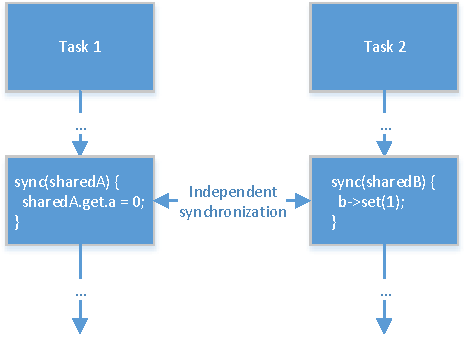
\includegraphics[scale=.9]{pics/ParallelExecution}
\end{minipage}

%. In this sense the synchronization itself is non-blocking which means that they will try to acquire the locks that are necessary in order to synchronize the access to the stated ressources. If this does not work they release all 

\subsection{Translation of shared types}
In order to fully understand the translation of synchronization statements the translation of shared types is given first. For the implementation of shared types in C two main solutions are conceivable which differ in the coupling that they exhibit between the data that is to be shared and the additional data required for access restriction, i.e. synchronization. In any case a solution must make use of additional data that can be used to synchronize two threads which try to read or write the shared data. To this end the most basic synchronization primitive, the mutex was chosen: each protected data item is assigned exactly one. 

In the first solution the data to be shared is stored as if no protection scheme existed, at all. Additionally all mutexes that are created by the application are stored in one global map which indexes each mutex by the memory address of its corresponding shared datum. This approach offers the advantage that access to the data itself is not influenced by the mutex protection: Every reference to the value of a shared ressource \CODE{e.get} can directly be translated into a reference to the wrapped value. Additionally, since the mutexes are globally managed all data that is returned by a library can be easily made (pseudo-) synchronization safe: E.g. if a pointer to an arbitrary memory location \texttt{loc} is returned the pointed-to address can be used to create a new mutex and add a mapping to the global mutex map. However, this on-the-fly protection of memory locations can incur synchronization leaks: The compiler cannot guarantee that addresses returning functions with unknown implementation will not leak their returned values to some other computation which accesses the according memory unsynchronized. This implies that such protection would only be safe if any reference to \texttt{loc} was wrapped in some shared ressource which in this scenario is not feasible. Hence, the design was chosen to not allow for such protection and consequently a global map would not be beneficial in this regard. A map solution would entail a space-time tradeoff. For illustrative purposes consider Google's C++ \textit{dense\_hash\_map} \footnote{http://goog-sparsehash.sourceforge.net/doc/dense\_hash\_map.html} which provides comparatively fast access to its members but imposes additional memory requirements to slower hashmap implementations\footnote{http://incise.org/hash-table-benchmarks.html}. An issue of hashmaps is the non-deterministic performance\footnote{Although real-time applications with their time-wise constraints are not a primary concern of this work it should nevertheless be kept in mind that they are part of the embedded domain. Therefore a solution that considers the characteristics of this domain is at least regarded advantageous.} and increased access time that may be induced by hash collisions\cite{FastAndDeterministicHashTable}.

The second solution for the implementation of shared types keeps each shareable datum and its mutex together: An instance of a struct with member fields for both components is used in place of the bare datum to be shared. In contrast to the aforementioned solution a reference to the value \CODE{e.get} needs one level of indirection via the struct instance. On the contrary the access to a mutex is simplified. As with the value it can be retrieved by a member access to the corresponding struct field whereas the map solution requires a map lookup to get the mutex (plus additional delay to make any modifying access to the map thread-safe). The computational overhead imposed by a struct member lookup is deemed negligible in the overall application performance. On the other hand the space required for the struct equals that of the individual fields plus additional padding\cite[pp.~303 ff.]{LinuxSystemProgramming} that is required to arrange the struct fields along valid memory addresses. The latter depends on the size of the data to be stored. In order to keep the padding as small as possible smart member ordering should be applied. 

For this work the struct solution was chosen in order to keep the access time of mutex lookups small and deterministic while not imposing too much space overhead and datum lookup overhead. For each kind of shared type \CODE{shared<t>} with the translated basetype \CODE{t'} a separate struct is generated:
\begin{ccode}
struct SharedOf_t {
  pthread_mutex_t mutex;
  t' value;
}
\end{ccode}
Any nested shared types are, hence, translated first. For implementation reasons nested \textit{typedef}s and constants used in array types are also resolved in this process\footnote{Although the resolution of typedefs and constants impedes corresponding (testwise) adjustment made by the programmer in the translated C code this is not deemed an issue since generally changes should always be made from within mbeddr, i.e. on the original code.}. Depending on the base type of the shared type the generated struct declaration is stored either in a generic module or in a newly generated other module: Consider the tree for a type \CODE{shared<t>} whose nodes are made of types and whose edges are formed by the base type relationship of shared types, array types and pointer types\footnote{Clearly, this tree will have only one branch.}, e.g: 


\begin{minipage}{0.3\textwidth}
\begin{ccode}
struct A { int32 val; }
shared<shared<A[10][20]>*>
\end{ccode}
\end{minipage}
\begin{minipage}{0.3\textwidth}
\begin{center}
\quad$\Longrightarrow$\qquad

the simplified type AST
\end{center}
\end{minipage}
\begin{minipage}{0.5\textwidth}
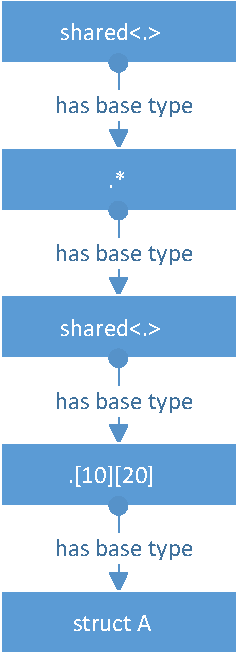
\includegraphics[scale=0.7]{pics/AstForBaseTypes}
\end{minipage}

\vspace{0.5cm}
If the leave of the tree is a primitive C type the struct declaration is stored in a generic module. In any other case the leave must be some struct type \CODE{s}. In order to preserve the visibility of the corresponding struct in the newly generated struct \CODE{SharedOf\_t} the latter is stored in the same module. Since the generation of code related to shared types can diminish the legibility of the resulting code profoundly for every such module a specific \textit{SharedTypes\_X} module is created and imported into the module that declares \CODE{s}. \textit{SharedTypes\_X} is used to store struct declarations like \CODE{SharedOf\_t}. Furthermore \CODE{s} is lifted into it in order to make it visible in the member declaration \CODE{value} of \CODE{SharedOf\_t}. For any field of \CODE{s} whose type tree contains another user-defined struct type the corresponding struct declaration is either lifted, as well (and recursively treated in the same way) or imported by its module. Should this separation of generated code used for shared type declarations and other user-defined code not proof well in praxis it could easily be deactivated.
With the former generation of the struct declaration in mind a type \CODE{shared<t>} is reduced to:
\begin{ccode}
SharedOf_t
\end{ccode}
The reduction of an expression \CODE{e.get} and \CODE{e.set(f)} make use of the \CODE{value} field of the \CODE{SharedOf\_t} struct. They are basically reduced to a retrieval of, respectively an assignment to the field:

\begin{minipage}{0.15\textwidth}
\begin{ccode}
e'.value
\end{ccode}
\end{minipage}
\begin{minipage}{0.2\textwidth}
respectively
\end{minipage}
\begin{minipage}{0.3\textwidth}
\begin{ccode}
e'.value = f'
\end{ccode}
\end{minipage}

If \CODE{e'} is has a pointer type the expressions \CODE{e->get} and \CODE{e->set(f)} are reduced to:

\begin{minipage}{0.15\textwidth}
\begin{ccode}
e'->value
\end{ccode}
\end{minipage}
\begin{minipage}{0.2\textwidth}
respectively
\end{minipage}
\begin{minipage}{0.3\textwidth}
\begin{ccode}
e'->value = f'
\end{ccode}
\end{minipage}

The mutex of the struct \CODE{SharedOf\_t} in the equally named struct field \CODE{mutex} which is used to synchronize one variable of an according type  must be initialized prior to any usage. This is done implicitly by generated code in order to free the programmer from this task. Accordingly, mutexes must be released before they get out of scope in order to prevent memory leaks. In the generated code both functionalities make use of corresponding functions, i.e. for every type who is one of the following types a pair of \CODE{mutexInit}--\CODE{mutexDestroy} functions is generated:

\begin{itemize}
\item shared types whose base types are shared types or for whom mutex functions are recursively generated;
\item array types who are not base types of array types themselves and whose base types are either shared types or struct types for whom mutex functions are recursively generated;
\item struct types whose structs contain at least one field with a type for which the same relation holds as for the aforementioned types.
\end{itemize}

For example, a type \CODE{shared<int32>[42][24]} would enforce the generation of one mutex initialization and one mutex destruction function. \CODE{shared<int32>*} on the other hand would not which makes sense as any variable \CODE{v} of this type would only point to a shared ressource which must be referenced directly by another variable \CODE{v'} of type \CODE{shared<int32>} or be contained in the memory-addressable value of some variable \CODE{v''} of a more complex type. The declaration of \CODE{v'}, respectively \CODE{v''} would then trigger the initialization of the mutex of the shared ressource that \CODE{v} points to. The resulting mutex initialization functions for types of the aforementioned kind are declared as follows:

\begin{ccode}
// for a proper shared type shared<t> and the type t' that t is reduced to
void mutexInit_X(SharedOf_t'* var) { 
  pthread_mutex_init(&var->mutex, &mutexAttribute);
  
  // either if t is a shared type or a struct type:
  mutexInit_X'(&var->value); 
  
  // or if t is an array type t[i_1]...[i_n] of 1 to n dimensions:
  mutexInit_X'((SharedOf_t'*...*)var->value, i_1, ..., i_n); 
}
\end{ccode}
For a shared ressource first the mutex of the corresponding translated struct is initialized by a call to the POSIX function \CODE{pthread\_mutex\_init()} which takes a mutex pointer and a mutex attribute pointer\footnote{The meaning of the mutex attribute will be explained later on.}. Then---since the shared ressource contains by aforementioned conditions another shared ressource---a call to the appropriate mutex function for the contained value is triggered. Depending on whether the base type of the current shared type is an array additional the dimension sizes for this base type may need to be provided as well (see below for details).

\begin{ccode}
// for a proper array type t[]...[] of 1 to n dimensions where ... denotes the occurrence of accordingly many symbols 
// and t' denotes the reduced-to type
void mutexInit_X(t'*...* var, int32 size_0, ..., int32 size_n) { 
  for (int32 __i_0 = 0; __i_0 < size_0; __i_0++) { 
    ...
      for (int32 __i_n = 0; __i_n < size_n; __i_n++) {
        // in case t is a struct type
        mutexInit_X'(&var[__i_0]...[__i_n]);
        
        // or, in case t is a shared type with generic C base type:
        pthread_mutex_init(&var[__i_0]...[__i_n].mutex, &mutexAttribute);
      }
    ...
  } 
}
\end{ccode}
For shared ressoures that are nested in arrays a nested iteration over all elements of the corresponding possibly multidimensional array with calls to either the generated mutex functions or the function defined by the POSIX standard are triggered.

For structs with nested shared ressources for each field that is or contains a shared ressource either the \CODE{pthread\_mutex\_init()} function is called directly or the mutex initialization is done by a call to the already generated function that is type compatible with this field (by possibly providing additional array dimensions):

\begin{ccode}
// for a proper struct type t of a struct t { u_1 f_1; ...; u_n f_n } and according reduced field types u_1' to u_n'
void mutexInit_X(SharedOf_t* var) {
  ...
  // in case u_i demands further initialization and it is a struct type or a shared type
  mutexInit_X'(&var->f_i);
  
  // in case u_i demands further initialization and it is an array type u_i[j_1]...[j_n] of 1 to n dimensions:
  mutexInit_X'((SharedOf_u_i'*...*)var->f_i, j_1, ..., j_n);
  
  // or, in case u_i is a shared type with generic C base type:
  pthread_mutex_init(&var->f_i.mutex, &mutexAttribute);
  ...
}
\end{ccode}
The signature of \CODE{mutexInit\_X()} for arrays shows that those are not passed as arrays to the mutex functions but as pointers. This is due to the necessity of declaring multidimensional arrays at least partially with the size for each dimension (e.g. \CODE{int[][]} would be missing at least one dimension size). Nevertheless it would not make sense to declare one mutex function for each shape of dimension size. Since arrays are treated like pointers internally when they are passed as function arguments it is completely safe to cast them to appropriate pointer types and to equally type the according function parameters.
The deletion of mutexes is defined quite similar to the initialization with the main difference that the utilized according pthreads function only takes one mutex. Therefore only the deletion for mutexes nested in ressources of shared types is shown:
\begin{ccode}
void mutexDestroy_X(SharedOf_t'* var) { 
  pthread_mutex_destroy (&var->mutex); 
  // ... further call to a mutexDestroy_X function equivalently to mutexInit_X shown above
}
\end{ccode}
The presented functions are used to initialize mutexes at the begin of their life span and delete them right before the corresponding end. For mutexes refered to by global variables this means that they must be initialized at the beginning of the entry function of the program\footnote{Due to the way mutexes are used in ParallelMbeddr (recursively---look below---and nested in structs) and the peculiaraties of C and the POSIX standard there is no way to combine the definition and the initialization of mutexes.}. As forced by mbeddr the programmer thus has to specify a main function in one of the implementation modules. Similarly mutexes of local variables are initialized right after their declaration whereas mutexes of function arguments are declared at the beginning of the related function\footnote{\label{mutexCopies}The possibility to have function arguments which contain or are shared ressources and, hence mutexes is not an obvious design choice: C's pass-by-value semantics of function parameters causes parameters to be copied into functions. Therefore a shared ressource which is not passed by its addresses but by its actual value will provoke the generation of an equal shared ressource at the beginning of the function execution. This copy is synchronization-wise completely unrelated to the original shared ressource since by the mutex copies cannot be used to lock with their origins\cite{Mutexes}. Furthermore they have to be initialized and destroyed seperately. The use of shared ressources in such a manner can confuse programmers who are not aware of this fact. Nevertheless ParallelMbeddr allows this kind of utilization of shared ressources in order to not burden the programmer with having to copy large structs that contain shared ressources component-wise if the shared ressource data is not of relevance. Depending on the feedback of future users it should be considered whether warnings for unintended misuse of shared ressources in this way might be helpful.}. The deletion of mutexes for shared ressources must be accomplished before they get out of scope which, again, depends on the kind of variables they are refered to. 
\TODO{Markus fragen, ob immer per main-Fkt. eingestiegen wird und ob Bibliotheksverwendung auch moeglich ist}
%Mutexes for global variables must be deleted at the end of the entry function of the program and before any return 
The mutexes of local variables must be destroyed before they get out of scope. Hence, mutex destruction calls are added at the end of their surrounding scopes if there is no control flow breaking statement (\textit{return}, \text{break}, \textit{continue}, \textit{goto}) as such cases are covered by the following rules. Take any control flow breaking statement \textit{c} that occurs in the AST of the same function as the declaration \textit{l} of some local variable does which refers to a (nested) shared ressource. If \textit{c} is part of the AST of any statement that follows \textit{l}\footnote{In other words: Consider only those control flow breaking statements \textit{c}s that are either one of the statements \textit{stmt}s which have the same AST parent \textit{p} and follow \textit{l} in the statement list of \textit{p} or are contained in the AST of some \text{stmt}} and
\begin{itemize}
\item \textit{c} is a \textit{return} statement and refers to a function or a closure whose AST contains \textit{l};
\item \textit{c} is a \textit{break} statement and refers to a loop or a \textit{switch} statement case whose AST contains \textit{l};
\item \textit{c} is a \textit{continue} statement and refers to a loop whose AST contains \textit{l};
\item \textit{c} is a \textit{goto} statement and refers to a label outside the AST of any statement that follows \textit{l}
\end{itemize}
\textit{c} must be preceded with a destruction call of the mutex of the shared ressource of \textit{l} (compare with the synchronization stopping rules below). The proper destruction of a mutex of an argument of function \textit{f} on the other hand just requires according function calls at the end of \textit{f} and before any return statement that refers to \textit{f}. 
Like inside the declarations of the mutex destruction functions explained above  the actual function to call for a variable or argument is either one of the \CODE{mutexDestroy\_X()} functions or a direct call of \CODE{pthread\_mutex\_destroy()} for ``simple'' shared ressources of generic C types, e.g.:
\begin{center}
\begin{minipage}{0.3\textwidth}
\begin{ccode}
// simple shared ressource
shared<int32> v1;

// complex shared ressource
shared<int32>[2][3] v2;
\end{ccode}
\end{minipage}
\qquad$\Longrightarrow$\qquad\qquad
\begin{minipage}{0.4\textwidth}
\begin{ccode}
SharedOf_int32_0 v1;
pthread_mutex_init(&v1.mutex, &mutexAttribute);

SharedOf_int32_0[2][3] v2;
mutexInit_0((SharedOf_int32_0**)v2, 2, 3);
\end{ccode}
\end{minipage}
\end{center}

To recap: The mutex of a shared ressource is either directly initiliazed and destroyed via appropriate pthreads functions or it is indirectly handled via functions that are based on the types of the values that shared ressources are nested inside. This approach was chosen in order to reduce the amount of code duplication that would otherwise occur if mutexes of shared ressources would be handled inline for every according variable. As a result the generated code's readibility is enhanced. The additional computational overhead due to function calls and returns should be regarded as an optimization concern of a further compilation step by a compiler like \textit{gcc}\TODO{or: by the compiler gcc}.
\TODO{Pruefen, ob mutex-init-Reihenfolge richtig ist}
ParallelMbeddr does not prevent the programmer from structuring the synchronization statements in such a way that a task will synchronize a shared variable multiple times (\textit{recursive synchronization}). The following code depicts such behavior:
\begin{ccode}
shared<int32> sharedValue;
sync(sharedValue) {
  sync(sharedValue) {
    sharedValue.set(42);
  }
}
\end{ccode}
Since each synchronization statement locks the mutexes of the refered shared ressources (see below for details) a recursive synchronization results in a \textit{recursive lock} of the corresponding mutex. Mutexes as defined by the POSIX standard must be specifically initialized in order to allow for this behavior\footnote{By default a recursive lock results in undefined behaviour because a default mutex does not have a lock count which is required to make recursive locks work: http://linux.die.net/man/3/pthread\_mutex\_trylock}: A mutex attribute that specifies the recursiveness must be defined and initialized first. It can then be used by arbitrarily many mutexes. 
For this purpose an application-wide attribute is defined in a generic module that is imported by all user-defined modules. It is initialized at the beginning of the main function:
\begin{ccode}
// inside the generic module:
pthread_mutexattr_t mutexAttribute
// at the beginning of main:
pthread_mutexattr_settype(&mutexAttribute, PTHREAD_MUTEX_RECURSIVE);
pthread_mutexattr_init(&mutexAttribute);
\end{ccode}

\subsection{Translation of synchronization statements}
Every synchronization statement is reduced to its statement list---as a block---surrounded with calls to functions that control the synchronization of the mutexes. The reduction for such a statement is given by either

\begin{center}
\begin{minipage}{0.3\textwidth}
\begin{ccode}
sync(e) stmt_list
\end{ccode}
\end{minipage}
\qquad$\Longrightarrow$\qquad\qquad\qquad
\begin{minipage}{0.4\textwidth}
\begin{ccode}
startSyncFor1Mutex(&e.mutex);
stmt_list'
stopSyncFor1Mutex(&e.mutex);
\end{ccode}
\end{minipage}
\end{center}

in case it contains only one synchronzied ressource, or else by

\begin{center}
\begin{minipage}{0.3\textwidth}
\begin{ccode}
sync(e_1, ..., e_n) stmt_list
\end{ccode}
\end{minipage}
\qquad$\Longrightarrow$\qquad\qquad\qquad
\begin{minipage}{0.4\textwidth}
\begin{ccode}
startSyncForNMutexes(&e_1.mutex, ..., &e_n.mutex);
stmt_list'
stopSyncForNMutexes(&e_1.mutex, ..., &e_n.mutex);
\end{ccode}
\end{minipage}
\end{center}

The statements are kept inside their statement list block in order to keep the scope of local variables inside synchronization statements. A synchronization statement list block is reduced to another block where statements that break the program flow structure may be preceded by an identical call of the \CODE{stopSyncForNMutexes()} function as is present after the list: Let \textit{s} be a synchronization statement and \textit{c} be a control flow breaking statement which is nested on some level in the AST of \textit{s}' statement list. Then \textit{c} is preceded with a call to \CODE{stopSyncForNMutexes()} if one of the following cases hold:
\begin{itemize}[label=]
\item \textit{c} is a \textit{return} statement and refers to a function or a closure whose AST contains \textit{s};
\item \textit{c} is a \textit{break} statement and refers to a loop or a \textit{switch} statement case whose AST contains \textit{s};
\item \textit{c} is a \textit{continue} statement and refers to a loop whose AST contains \textit{s}.
\item \textit{c} is a \textit{goto} statement and refers to a label outside the AST of \textit{s}.
\end{itemize}

In this manner inconsistent synchronization states of shared ressources due to a control flow break by the aforementioned statements are omitted. Since the occurrence of such a statement may also force ParallelMbeddr to insert \CODE{mutexDestroy\_X()} calls a careless mixture of mutex unlocking and destruction calls can cause runtime errors\cite{Mutexes}. The generator therefore takes care of putting any destruction calls behind the generated unlocking calls.

For each arity of synchronization ressources seperate versions of the \CODE{start}- and \CODE{stopSyncForNMutexes()} functions are declared inside a generic C module. A \CODE{stopSyncForNMutexes()} function straightforwardly redirects its mutex parameters to calls of the \CODE{pthread\_mutex\_unlock} function:
\begin{ccode}
// the corresponding function 'stopSyncFor1Mutex()' for exactly one mutex is skipped, here
void stopSyncForNMutexes(pthread_mutex_t* mutex_1, ..., pthread_mutex_t* mutex_n) { 
  pthread_mutex_unlock (mutex_1);
  ...
  pthread_mutex_unlock (mutex_n); 
}
\end{ccode}

Abstracted over the details of the actual implementation, synchronization statements synchronize their ressources atomically as was mentioned in the preceding design section. Since one or more mutexes can be tentatively locked by multiple threads simultaneously specific contention management has to be taken care of. The illusion of atomic synchronization is realized by an implementation of the obstruction-free\footnote{Busy-waiting means that the thread will repeatedly test a condition until it is met, without doing actual useful work\cite[p.~166]{AnIntroductionToParallelProgramming}. Thus, it is an alternative to suspending a thread and revoking it later on when some condition is met (which can, e.g., be realized by \textit{condition variables} as provided by POSIX threads\cite[p.~77]{ProgrammingWithPOSIXThreads}). Obstruction-free means that the execution of any thread which is at some time run in isolation such that the execution of obstructing other threads is interrupted meanwhile will progress. The existance of obstruction-freedom guarantees that no deadlocks will occur\cite{ObstructionFreeAuthorizationEnforcement}. However, livelocks and starvation are not necessarily avoided. Stronger degrees of non-blocking algorithms like lock-freedom and wait-freedom tackle these problems (partially) but are not relevant for this work. Further information on the latter is for instance provided by http://preshing.com/20120612/an-introduction-to-lock-free-programming/. %http://doc.akka.io/docs/akka/snapshot/general/terminology.html
} busy-wait protocol \textit{Polite}. In order to resolve conflicts \textit{Polite} uses exponential backoff. The according backoff function is explained further down. The synchronization function tries to lock every mutex as given by its arguments. On failure it releases every mutex that was locked so far, uses the backoff function to delay its execution for a randomized amount of time and repeats afterwards. This scheme enables competing threads to (partially) proceed and avoid deadlocks due to unordered overlapping mutex locks\footnote{Again, the presented scheme does not prevent the programmer from nesting the synchronization statements in such a manner that deadlocks in nested synchronization statements occur. It is rather a prevention of deadlocks that are caused solely by synchronization statements on the same nesting level.}.
\begin{ccode}
// again, the equivalent function declaration for 1 mutex is skipped
void startSyncForNMutexes(pthread_mutex_t* mutex_0, ..., pthread_mutex_t* mutex_m, pthread_mutex_t* mutex_n) { 
  uint8 waitingCounter = 0; 
  uint16 mask = 16; 
  uint32 seed = (uint32)(uintptr_t) &waitingCounter;
  
  while (true) { 
    if ([| pthread_mutex_trylock (mutex_0) |] != 0) { 
      backoffExponentially(&waitingCounter, &mask, &seed); 
    } 
    else if ([| pthread_mutex_trylock (mutex_1) |] != 0) { 
      [| pthread_mutex_unlock (mutex_0) |]; 
      backoffExponentially(&waitingCounter, &mask, &seed); 
    } ...
    else if ([| pthread_mutex_trylock (mutex_n) |] != 0) { 
      [| pthread_mutex_unlock (mutex_m) |];
      ...
      [| pthread_mutex_unlock (mutex_0) |]; 
      backoffExponentially(&waitingCounter, &mask, &seed); 
    } 
    else { 
      break; 
    } 
  }
}
\end{ccode}

The backoff realized by Polite randomizedly delays the execution  by less than \textit{limit} $ = 2^{n+k}$ ns\cite{AdvancedContentionManagement}. \textit{n} denotes the retry counter and \textit{k} denotes some constant offset which can be machine-tuned. The randomized wait time of the exponential backoff is used to avoid livelocks which could happen if two threads would repeatedly compete for the same ressources and delay their execution for equal amounts of time. In the current implementation \CODE{backoffExponentially()} of the contention management the offset \textit{k} is set to 4 and a threshold \textit{m} of 17 denotes the number of rounds after which \textit{k} is reset\footnote{\textit{k}'s value is reflected in the initial value ($2^4 = 16$) of \CODE{mask} whereas \textit{m}'s value is composed of mask's base and the divisor (13) in the calculation of the next \CODE{waitingCounter}.}. Thus, maximum delays of about 100 ms (specifically 131 ms) are allowed\footnote{The search for machine- or application-specific optimal offsets and thresholds is a task for future enhancements of ParallelMbeddr.}. 
\begin{ccode}
inline void backoffExponentially(uint8* waitingCounter, uint16* mask, uint32* seed) { 
  *mask |= 1 << *waitingCounter; 
  randomWithXorShift(seed); 
  struct timespec sleepingTime = (struct timespec){ .tv_nsec = *seed & *mask }; 
  nanosleep(&sleepingTime, null); 
  *waitingCounter = (*waitingCounter + 1) % 13; 
}
\end{ccode}
Note that \CODE{backoffExponentially()} keeps its main state inside the \CODE{startSyncForNMutexes()} function. The state will therefore be re-initialized before the execution of every synchronization block. The generation of the pseudo-randomized delay is realized via utilization of the Marsaglia's Xorshift random number generator\cite{XorshiftRngs}:
\begin{ccode}
void randomWithXorShift(uint32* seed) { 
  *seed ^= *seed << 13; 
  *seed ^= *seed >> 17; 
  *seed ^= *seed << 5; 
}
\end{ccode}
The generator was chosen for its high performance, low memory consumption and thread safety due to the utilization of the stack-managed \CODE{seed} parameter as opposed to the global state usage of the standard C random generator \CODE{rand()}. The fact that after a certain number---which may be smaller than in other generators---of repeated calls with the same seed value (i.e. the same memory address of a seed) repetitions of the sequence of calculated numbers will occur is not of relevance for the purpose of this work.

\subsection{Example code}
In the previous sections \ref{taskExample} and \ref{futuresExample} the running example approximated the number $\pi$ by using tasks which calculate exactly one fraction of the result each and retrieving their results via futures. The amount of work was therefore partitioned in advance. In this section a more dynamic approach is chosen instead: The work of every task comprises major and minor rounds. A minor round is equivalent to the full calculation loop in the previous $\pi$ solution. In every step of a major round initiatiates a minor round by first coordinating with the other tasks which range of $\pi$ it should calculate. After having calculated the sum in a minor round the task then uses a queue to store its next partial result. A dedicated task is used to collect these partial results from the queue and accumulate them to a complete sum which in the end is the result of the over-all approximated $\pi$. The communication-based solution can be seen as a map-reduce implementation where partial results a mapped onto the queue by a certain number of tasks and from there reduced to a final result by a seperate task (compare with \cite{MapReduce}).
